\subsection{Credit card dataset}
This dataset includes two classes, highly unbalanced: fraud or not fraud.
\subsubsection{Subtractive clustering}
    In Tables \ref{tab:c1_n_s}, \ref{tab:c2_n_s} and \ref{tab:ce_n_s} are shown the number of clusters found for the three datasets of credit card fraud. In this case, we observe that the cosine norm achieves 2 clusters, the expected ones. But probably more clusters are not a wrong performance, rather than a different form of viewing the data. We will refer then to the validation indices to see when the performance is better. Also, in Figure~\ref{fig:credit_s_i} is shown the initial density function for the credit card reduced dataset and $r_a = 0.5$, with the euclidean distance. Figure~\ref{fig:credit_s_f} shows the final state.
    \begin{table}[ht!]
        \centering
        \begin{tabular}{lrrr}
        \toprule
        $r_a$ &  euclidean &  cosine &  cityblock \\
        \midrule
        0.4 &         10 &       2 &         52 \\
        0.5 &          7 &       2 &         21 \\
        0.7 &          4 &       2 &          8 \\
        \bottomrule \\
        \end{tabular}
        \caption{Number of clusters found by the subtractive algorithm for the credit card dataset.}
        \label{tab:c1_n_s}
    \end{table}
    
    \begin{table}[ht!]
        \centering
        \begin{tabular}{lrrr}
        \toprule
        $r_a$ &  euclidean &  cosine &  cityblock \\
        \midrule
        0.4 &          8 &       2 &         23 \\
        0.5 &          5 &       2 &         11 \\
        0.7 &          3 &       2 &          5 \\
        \bottomrule \\
        \end{tabular}
        \caption{Number of clusters found by the subtractive algorithm for the credit card reduced dataset.}
        \label{tab:c2_n_s}
    \end{table}
    
    \begin{table}[ht!]
        \centering
        \begin{tabular}{lrrr}
        \toprule
        $r_a$ &  euclidean &  cosine &  cityblock \\
        \midrule
        0.4 &         99 &       8 &         99 \\
        0.5 &         99 &       7 &         99 \\
        0.7 &         99 &       4 &         99 \\
        \bottomrule \\
        \end{tabular}
        \caption{Number of clusters found by the subtractive algorithm for the credit card embbeded dataset.}
        \label{tab:ce_n_s}
    \end{table}
    
    The algorithm has an emergency stopping criteria, the number of iterations. Due to the fact that they are 100, is clear that for the euclidean distance in the embbeded dataset much more clusters are achieved. This may be due to the spatial distribution of the data, as shwon in the results of Figure~\ref{fig:credit_s}.
    
    \begin{table}[ht!]
        \centering
        \begin{tabular}{lrrr}
        \toprule
        $r_a$ &  euclidean &    cosine &  cityblock \\
        \midrule
        0.4 &   3.029305 &  0.981477 &   3.374885 \\
        0.5 &   3.441991 &  0.981142 &   3.349646 \\
        0.7 &   3.737428 &  0.981221 &   4.300733 \\
        \bottomrule \\
        \end{tabular}
        \caption{Davies Bouldin index for the credit card dataset clustered by the subtractive algorithm.}
        \label{tab:c1_db_s}
    \end{table}
    
    \begin{table}[ht!]
        \centering
        \begin{tabular}{lrrr}
        \toprule
        $r_a$ &     euclidean &         cosine &     cityblock \\
        \midrule
        0.4 &  34200.815670 &  181518.597459 &   4712.546985 \\
        0.5 &  45858.080636 &  181504.729539 &  10983.494778 \\
        0.7 &  67334.688094 &  181520.031384 &  30413.670844 \\
        \bottomrule \\
        \end{tabular}
        \caption{Calisnki-Harabsz score for the credit card dataset clustered by the subtractive algorithm.}
        \label{tab:c1_ch_s}
    \end{table}
    
    In Tables \ref{tab:c1_db_s} and \ref{tab:c1_db_s} are shown the results for the validation of the clustering in the original credit card dataset. We saw that, for the cosine metric the number of clusters found are the expected, and is actually revised by these scores, that classify this metric as the one that performs the better. \\
    
    \begin{table}[ht!]
        \centering
        \begin{tabular}{lrrr}
        \toprule
        $r_a$ &  euclidean &    cosine &  cityblock \\
        \midrule
        0.4 &   2.409494 &  0.875412 &   3.139200 \\
        0.5 &   2.088824 &  0.875412 &   2.601788 \\
        0.7 &   1.468652 &  0.875644 &   3.157173 \\
        \bottomrule \\
        \end{tabular}
        \caption{Davies Bouldin index for the credit card reduced dataset clustered by the subtractive algorithm.}
        \label{tab:c2_db_s}
    \end{table}
    
    \begin{table}[ht!]
        \centering
        \begin{tabular}{lrrr}
        \toprule
        $r_a$ &      euclidean &         cosine &     cityblock \\
        \midrule
        0.4 &   47725.987561 &  210512.707501 &  12023.907405 \\
        0.5 &   92681.517486 &  210512.707501 &  31914.695617 \\
        0.7 &  113693.471190 &  210511.841004 &  59832.246699 \\
        \bottomrule \\
        \end{tabular}
        \caption{Calisnki-Harabsz score for the reduced credit card dataset clustered by the subtractive algorithm.}
        \label{tab:c2_ch_s}
    \end{table}
    
    In Tables \ref{tab:c2_db_s} and \ref{tab:c2_ch_s} are shown the indices for the reduced dataset by PCA. Again, the performance shown by these corresponds to the fact that the cosine metric achieves the expected number of clusters.
    
    \begin{table}[ht!]
        \centering
        \begin{tabular}{lrrr}
        \toprule
        $r_a$ &  euclidean &    cosine &  cityblock \\
        \midrule
        0.4 &   1.080875 &  1.176533 &   1.253805 \\
        0.5 &   1.050448 &  1.093338 &   1.333077 \\
        0.7 &   0.953949 &  0.866116 &   1.043586 \\
        \bottomrule \\
        \end{tabular}
        \caption{Davies Bouldin index for the credit card embbeded dataset clustered by the subtractive algorithm.}
        \label{tab:ce_db_s}
    \end{table}
    
    \begin{table}[ht!]
        \centering
        \begin{tabular}{lrrr}
        \toprule
        $r_a$ &      euclidean &         cosine &      cityblock \\
        \midrule
        0.4 &   83056.373617 &  174368.043596 &   77677.563496 \\
        0.5 &  109156.916197 &  185793.584797 &   88929.724177 \\
        0.7 &  142020.902180 &  217192.867615 &  116444.149920 \\
        \bottomrule \\
        \end{tabular}
        \caption{Calisnki-Harabsz score for the reduced credit card dataset clustered by the subtractive algorithm.}
        \label{tab:ce_ch_s}
    \end{table}
    
    Finally, Tables \ref{tab:ce_db_s} and \ref{tab:ce_ch_s} are shown the validity indices or the embbeded dataset. These indices show a poor performance in all cases, reflecting the amount of clusters found by the algorithm in this particular dataset. Probably, the information given by the embbeding is not enough to show the full structure of the data.
    
    \begin{figure}[ht!]
        \centering
        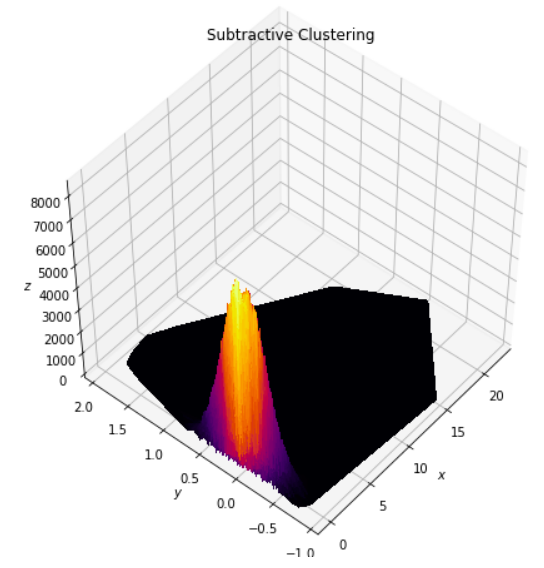
\includegraphics[scale = 0.4]{figures/credit/credit_s_i.png}
        \caption{Initial density function for the credit card dataset in the subtractive clustering algorithm.}
        \label{fig:credit_s_i}
    \end{figure}
    
    \begin{figure}[ht!]
        \centering
        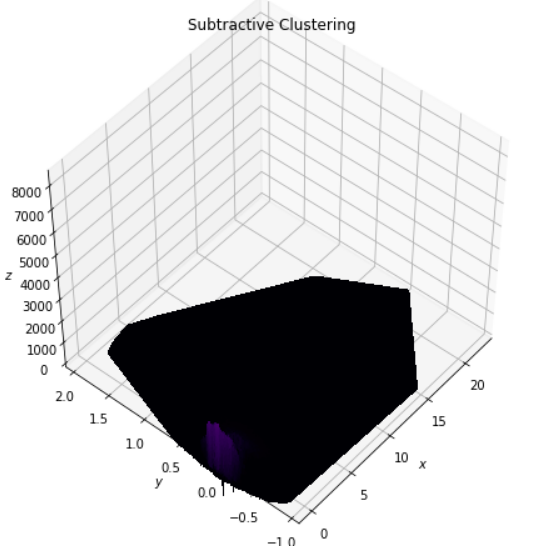
\includegraphics[scale = 0.4]{figures/credit/credit_s_f.png}
        \caption{Final density function for the credit card dataset in the subtractive clustering algorithm.}
        \label{fig:credit_s_f}
    \end{figure}
    
    \begin{figure}[ht!]
        \centering
        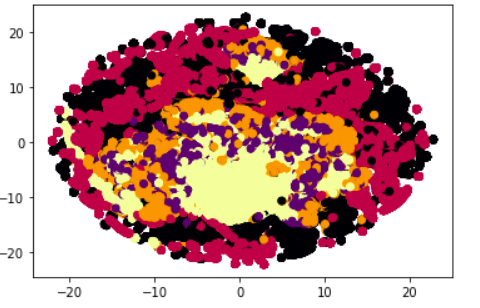
\includegraphics[scale = 0.4]{figures/credit/credit_s.png}
        \caption{Clustering for the credit card dataset in the subtractive clustering algorithm.}
        \label{fig:credit_s}
    \end{figure}
\subsubsection{Mountain clustering} Tables \ref{tab:c2_n_m} and \ref{tab:ce_n_m} show the number of clusters found by the mountain algorithm in the embbeded and reduced dataset, with variations in the smoothing paramenter $\sigma$ and the metric.

\begin{table}[ht!]
    \centering
   \begin{tabular}{lrrr}
    \toprule
    $\sigma$ &  euclidean &  cosine &  cityblock \\
    \midrule
    0.4 &          8 &       7 &          2 \\
    0.5 &          4 &       5 &          2 \\
    0.7 &          3 &       3 &          2 \\
    \bottomrule \\
    \end{tabular}
    \caption{Number of clusters found by the mountain algorithm in the reduced credit card dataset.}
    \label{tab:c2_n_m}
\end{table}

\begin{table}[ht!]
    \centering
    \begin{tabular}{lrrr}
    \toprule
    $\sigma$ &  euclidean &  cosine &  cityblock \\
    \midrule
    0.4 &         10 &       5 &          9 \\
    0.5 &          9 &       4 &         10 \\
    0.7 &          9 &       4 &          9 \\
    \bottomrule \\
    \end{tabular}
    \caption{Number of clusters found by the mountain algorithm in the embbeded credit card dataset.}
    \label{tab:ce_n_m}
\end{table}

In this case, we observe that the number of clusters is reduced in comparison with the subtractive algorithm, however, the metric that only finds the two existing clusters in the dataset is the manhattan, and only in the reduced one. The embbeded one, again, does not seem to provide enough information to perform a good clustering.

\begin{table}[ht!]
    \centering
    \begin{tabular}{lrrr}
        \toprule
        $\sigma$ &  euclidean &    cosine &  cityblock \\
        \midrule
        0.4 &   5.395964 &  2.539999 &   6.582867 \\
        0.5 &   5.076245 &  3.047503 &   6.582867 \\
        0.7 &   4.635804 &  1.861457 &   6.582867 \\
        \bottomrule \\
        \end{tabular}
    \caption{Davies Bouldin index for the reduced credit card dataset clustered by the mountain algorithm.}
    \label{tab:c2_db_m}
\end{table}

\begin{table}[ht!]
    \centering
    \begin{tabular}{lrrr}
    \toprule
    $\sigma$ &    euclidean &         cosine &    cityblock \\
    \midrule
    0.4 &  2612.705876 &   41225.158046 &  4029.893595 \\
    0.5 &  3689.213460 &   58473.394701 &  4029.893595 \\
    0.7 &  3966.374184 &  110716.512521 &  4029.893595 \\
    \bottomrule \\
    \end{tabular}
    \caption{Calinski-Harabasz score for the reduced credit card dataset clustered by the mountain algorithm.}
    \label{tab:c2_ch_m}
    \end{table}
    
    In Tables \ref{tab:c2_db_m} and \ref{tab:c2_ch_m} are shown the validity indices for the clustering in the reduced dataset.
    
\begin{table}[ht!]
    \centering
    \begin{tabular}{lrrr}
        \toprule
        $\sigma$ &  euclidean &    cosine &  cityblock \\
        \midrule
        0.4 &   0.891413 &  0.967157 &   0.946406 \\
        0.5 &   0.884992 &  0.878476 &   0.891413 \\
        0.7 &   0.884992 &  0.865683 &   0.884992 \\
        \bottomrule \\
        \end{tabular}
    \caption{Davies Bouldin index for the embbeded credit card dataset clustered by the mountain algorithm.}
    \label{tab:ce_db_m}
\end{table}

\begin{table}[ht!]
    \centering
    \begin{tabular}{lrrr}
        \toprule
        $\sigma$ &      euclidean &         cosine &      cityblock \\
        \midrule
        0.4 &  198415.832838 &  193511.849750 &  188520.438083 \\
        0.5 &  208251.768500 &  207307.628003 &  198415.832838 \\
        0.7 &  208251.768500 &  217172.104734 &  208251.768500 \\
        \bottomrule \\
        \end{tabular}
    \caption{Calinski-Harabasz score for the embbeded credit card dataset clustered by the mountain algorithm.}
    \label{tab:ce_ch_m}
\end{table}

\subsubsection{k-means clustering}
This method was implemented passing as a parameter ht number of clusters found by the subtractive and mountain clustering algorithms

\begin{table}[ht!]
    \centering
   \begin{tabular}{lrrr}
\toprule
$k$ &  euclidean &  cityblock &    cosine \\
\midrule
2  &   0.986952 &   0.969734 &  0.980718 \\
8  &   2.007106 &   3.722434 &  2.595858 \\
23 &   2.760027 &   3.213468 &  2.849296 \\
52 &   2.762716 &   3.225261 &  2.803379 \\
\bottomrule
\end{tabular}
    \caption{Davies Bouldin index for the credit card dataset clustered by the k-means algorithm.}
    \label{tab:c1_db_k}
\end{table}

\begin{table}[ht!]
    \centering
    \begin{tabular}{lrrr}
\toprule
$k$ &      euclidean &      cityblock &         cosine \\
\midrule
2  &  181436.153264 &  180730.956220 &  181557.762218 \\
8  &   98847.628899 &   53207.410205 &   39698.094090 \\
23 &   31137.058905 &   34841.417018 &   18892.562407 \\
52 &   24134.173179 &   22951.749474 &   13311.399645 \\
\bottomrule
\end{tabular}

    \caption{Calinski-Harabasz score for the credit card dataset clustered by the k-means algorithm.}
    \label{tab:c1_ch_k}
\end{table}

\begin{table}[ht!]
    \centering
     \begin{tabular}{lrrr}
\toprule
$k$ &  euclidean &  cityblock &    cosine \\
\midrule
2  &   0.877730 &   0.880508 &       NaN \\
8  &   2.024618 &   2.982872 &  3.328334 \\
23 &   2.619990 &   3.711084 &  3.178648 \\
52 &   2.864630 &   3.711084 &  3.178648 \\
\bottomrule
\end{tabular}
    \caption{Davies Bouldin index for the reduced credit card dataset clustered by the k-means algorithm.}
    \label{tab:c2_db_k}
\end{table}

\begin{table}[ht!]
    \centering
    \begin{tabular}{lrrr}
\toprule
$k$ &      euclidean &      cityblock &        cosine \\
\midrule
2  &  210529.106925 &  209875.102760 &           NaN \\
8  &   72946.792723 &   83930.170088 &  33612.695045 \\
23 &   59111.059374 &   43480.419564 &  37234.450527 \\
52 &   51906.683233 &   43480.419564 &  37234.450527 \\
\bottomrule
\end{tabular}
    \caption{Calinski-Harabasz score for the reduced credit card dataset clustered by the k-means algorithm.}
    \label{tab:c2_ch_k}
\end{table}

\begin{table}[ht!]
    \centering
    \begin{tabular}{lrrr}
\toprule
$k$ &  euclidean &  cityblock &    cosine \\
\midrule
2  &   1.228585 &   1.228108 &       NaN \\
8  &   1.207162 &   1.228173 &  1.233886 \\
23 &   1.207162 &   1.228173 &  1.233886 \\
52 &   1.207162 &   1.228173 &  1.233886 \\
\bottomrule
\end{tabular}
    \caption{Davies Bouldin index for the embbeded credit card dataset clustered by the k-means algorithm.}
    \label{tab:ce_db_k}
\end{table}

\begin{table}[ht!]
    \centering
   \begin{tabular}{lrrr}
\toprule
$k$ &      euclidean &      cityblock &         cosine \\
\midrule
2  &  154605.093889 &  153712.597451 &            NaN \\
8  &  149112.870073 &  152290.919907 &  153293.566791 \\
23 &  149112.870073 &  152290.919907 &  153293.566791 \\
52 &  149112.870073 &  152290.919907 &  153293.566791 \\
\bottomrule
\end{tabular}
    \caption{Calinski-Harabasz score for the embbeded credit card dataset clustered by the k-means algorithm.}
    \label{tab:ce_ch_k}
\end{table}

\subsubsection{c-means clustering}

\begin{table}[ht!]
    \centering
   \begin{tabular}{lrrr}
\toprule
$c$ &  euclidean &  cityblock &    cosine \\
\midrule
2  &   0.981125 &   0.981627 &  0.980810 \\
8  &   4.732980 &   6.635164 &  3.085351 \\
23 &  17.466621 &   9.915131 &  4.062041 \\
52 &  29.236820 &   7.124120 &  3.591925 \\
\bottomrule
\end{tabular}
    \caption{Davies Bouldin index for the credit card dataset clustered by the c-means algorithm.}
    \label{tab:c1_db_c}
\end{table}

\begin{table}[ht!]
    \centering
    \begin{tabular}{lrrr}
\toprule
$c$ &      euclidean &      cityblock &         cosine \\
\midrule
2  &  181559.515470 &  181523.468131 &  181557.965676 \\
8  &   49096.008959 &   26035.605235 &   35559.318512 \\
23 &   16145.589302 &    8283.743644 &   15358.374324 \\
52 &    7354.748555 &    3574.418012 &    7080.939622 \\
\bottomrule
\end{tabular}
    \caption{Calinski-Harabasz score for the credit card dataset clustered by the c-means algorithm.}
    \label{tab:c1_ch_c}
\end{table}

\begin{table}[ht!]
    \centering
     \begin{tabular}{lrrr}
\toprule
$k$ &  euclidean &  cityblock &    cosine \\
\midrule
2  &   0.877730 &   0.880508 &       NaN \\
8  &   2.024618 &   2.982872 &  3.328334 \\
23 &   2.619990 &   3.711084 &  3.178648 \\
52 &   2.864630 &   3.711084 &  3.178648 \\
\bottomrule
\end{tabular}
    \caption{Davies Bouldin index for the reduced credit card dataset clustered by the k-means algorithm.}
    \label{tab:c2_db_k}
\end{table}

\begin{table}[ht!]
    \centering
    \begin{tabular}{lrrr}
\toprule
$k$ &      euclidean &      cityblock &        cosine \\
\midrule
2  &  210529.106925 &  209875.102760 &           NaN \\
8  &   72946.792723 &   83930.170088 &  33612.695045 \\
23 &   59111.059374 &   43480.419564 &  37234.450527 \\
52 &   51906.683233 &   43480.419564 &  37234.450527 \\
\bottomrule
\end{tabular}
    \caption{Calinski-Harabasz score for the reduced credit card dataset clustered by the k-means algorithm.}
    \label{tab:c2_ch_k}
\end{table}

\begin{table}[ht!]
    \centering
    \begin{tabular}{lrrr}
\toprule
$k$ &  euclidean &  cityblock &    cosine \\
\midrule
2  &   1.228585 &   1.228108 &       NaN \\
8  &   1.207162 &   1.228173 &  1.233886 \\
23 &   1.207162 &   1.228173 &  1.233886 \\
52 &   1.207162 &   1.228173 &  1.233886 \\
\bottomrule
\end{tabular}
    \caption{Davies Bouldin index for the embbeded credit card dataset clustered by the k-means algorithm.}
    \label{tab:ce_db_k}
\end{table}

\begin{table}[ht!]
    \centering
   \begin{tabular}{lrrr}
\toprule
$k$ &      euclidean &      cityblock &         cosine \\
\midrule
2  &  154605.093889 &  153712.597451 &            NaN \\
8  &  149112.870073 &  152290.919907 &  153293.566791 \\
23 &  149112.870073 &  152290.919907 &  153293.566791 \\
52 &  149112.870073 &  152290.919907 &  153293.566791 \\
\bottomrule
\end{tabular}
    \caption{Calinski-Harabasz score for the embbeded credit card dataset clustered by the k-means algorithm.}
    \label{tab:ce_ch_k}
\end{table}

\subsection{k-medians clustering}

\begin{table}[ht!]
    \centering
   \begin{tabular}{lrrr}
\toprule
$k$ &  euclidean &  cityblock &    cosine \\
\midrule
2  &   0.961783 &   0.962315 &  0.980090 \\
8  &   2.628569 &   4.411534 &  2.590670 \\
23 &   2.868963 &   3.573171 &  2.812779 \\
52 &   2.636274 &   3.351422 &  2.770461 \\
\bottomrule \\
\end{tabular}
    \caption{Davies Bouldin index for the credit card dataset clustered by the k-medians algorithm.}
    \label{tab:c1_db_km}
\end{table}

\begin{table}[ht!]
    \centering
    \begin{tabular}{lrrr}
\toprule
$k$ &      euclidean &      cityblock &         cosine \\
\midrule
2  &  179819.801998 &  179538.695544 &  181537.864020 \\
8  &   59893.705373 &   32098.341423 &   39862.438248 \\
23 &   34637.384138 &   14599.172093 &   18145.362814 \\
52 &   26166.412507 &   23669.675506 &   14099.041695 \\
\bottomrule \\
\end{tabular}
    \caption{Calinski-Harabasz score for the credit card dataset clustered by the k-medians algorithm.}
    \label{tab:c1_ch_km}
\end{table}

\begin{table}[ht!]
    \centering
     \begin{tabular}{lrrr}
\toprule
$k$ &  euclidean &  cityblock &    cosine \\
\midrule
2  &   0.856449 &   0.859836 &  0.875516 \\
8  &   1.993958 &   4.636362 &  3.649393 \\
23 &   2.864630 &   3.711084 &  3.178648 \\
52 &   2.864630 &   3.711084 &  3.178648 \\
\bottomrule \\
\end{tabular}
    \caption{Davies Bouldin index for the reduced credit card dataset clustered by the k-medians algorithm.}
    \label{tab:c2_db_km}
\end{table}

\begin{table}[ht!]
    \centering
    \begin{tabular}{lrrr}
\toprule
$k$ &      euclidean &      cityblock &         cosine \\
\midrule
2  &  208109.035906 &  208524.442055 &  210505.933632 \\
8  &   84247.287201 &   55071.943951 &   58980.928613 \\
23 &   51906.683233 &   43480.419564 &   37234.450527 \\
52 &   51906.683233 &   43480.419564 &   37234.450527 \\
\bottomrule \\
\end{tabular}
    \caption{Calinski-Harabasz score for the reduced credit card dataset clustered by the k-medians algorithm.}
    \label{tab:c2_ch_km}
\end{table}

\begin{table}[ht!]
    \centering
    \begin{tabular}{lrrr}
\toprule
$k$ &  euclidean &  cityblock &    cosine \\
\midrule
2  &   1.228260 &        NaN &  1.234059 \\
8  &   1.207162 &   1.228173 &  1.233886 \\
23 &   1.207162 &   1.228173 &  1.233886 \\
52 &   1.207162 &   1.228173 &  1.233886 \\
\bottomrule \\
\end{tabular}
    \caption{Davies Bouldin index for the embbeded credit card dataset clustered by the k-medians algorithm.}
    \label{tab:ce_db_km}
\end{table}

\begin{table}[ht!]
    \centering
  \begin{tabular}{lrrr}
\toprule
$k$ &      euclidean &      cityblock &         cosine \\
\midrule
2  &  154686.549909 &            NaN &  153253.248913 \\
8  &  149112.870073 &  152290.919907 &  153293.566791 \\
23 &  149112.870073 &  152290.919907 &  153293.566791 \\
52 &  149112.870073 &  152290.919907 &  153293.566791 \\
\bottomrule \\
\end{tabular}

    \caption{Calinski-Harabasz score for the embbeded credit card dataset clustered by the k-medians algorithm.}
    \label{tab:ce_ch_km}
\end{table}